\documentclass{article}

% if you need to pass options to natbib, use, e.g.:
%     \PassOptionsToPackage{numbers, compress}{natbib}
% before loading neurips_2020

\usepackage{natbib}
\bibliographystyle{abbrvnat}
\setcitestyle{authoryear,open={(},close={)}}

% commands for comments
\usepackage[dvipsnames]{xcolor}
\newcommand{\todo}[1]{\textbf{\textcolor{Red}{(TODO: #1)}}}

% ready for submission
%\usepackage{neurips_2020}

% to compile a preprint version, e.g., for submission to arXiv, add add the
% [preprint] option:
    \usepackage[preprint]{neurips_2020}

% to compile a camera-ready version, add the [final] option, e.g.:
%  \usepackage[final]{neurips_2020}

% to avoid loading the natbib package, add option nonatbib:
%     \usepackage[nonatbib]{neurips_2020}

\usepackage[utf8]{inputenc} % allow utf-8 input
\usepackage[T1]{fontenc}    % use 8-bit T1 fonts
\usepackage[colorlinks,citecolor=blue]{hyperref}       % hyperlinks
\usepackage{url}            % simple URL typesetting
\usepackage{booktabs}       % professional-quality tables
\usepackage{amsfonts}       % blackboard math symbols
\usepackage{nicefrac}       % compact symbols for 1/2, etc.
\usepackage{microtype}      % microtypography
\usepackage{amsmath}
\usepackage{dcolumn}
\usepackage{makecell}
\usepackage{amssymb}
\usepackage{graphicx}		% include figures
\usepackage{tabularx}
\usepackage{float}			% keeps figures in place
\usepackage{xurl}           % keeps URL from overflowing
\usepackage{caption}
\captionsetup[table]{skip=10pt} % includes space between table and caption
\usepackage{subcaption}		% create subfigures

\newcolumntype{d}[1]{D{.}{.}{#1}} % "decimal" column type
\renewcommand{\ast}{{}^{\textstyle *}} % for raised "asterisks"


\title{Comparing Multimodal Representations in Co-Attention-Based Models for Visual Question Answering}

% The \author macro works with any number of authors. There are two commands
% used to separate the names and addresses of multiple authors: \And and \AND.
%
% Using \And between authors leaves it to LaTeX to determine where to break the
% lines. Using \AND forces a line break at that point. So, if LaTeX puts 3 of 4
% authors names on the first line, and the last on the second line, try using
% \AND instead of \And before the third author name.

\author{%
   Patrick Kahardipraja%\thanks{Use footnote for providing further information
    %about author (webpage, alternative address)---\emph{not} for acknowledging
    %funding agencies.} \\
  %Department of Computer Science\\
  %Cranberry-Lemon University\\
  %Pittsburgh, PA 15213 \\
  %\texttt{hippo@cs.cranberry-lemon.edu} \\
  % examples of more authors
  \And
   Laura Kopf \\
  % Affiliation \\
  % Address \\
  % \texttt{email} \\
  % \AND
  % Coauthor \\
  % Affiliation \\
  % Address \\
  % \texttt{email} \\
  % \And
  % Coauthor \\
  % Affiliation \\
  % Address \\
  % \texttt{email} \\
  % \And
  % Coauthor \\
  % Affiliation \\
  % Address \\
  % \texttt{email} \\
}

\begin{document}

\maketitle

%general question: should we write integers in text as "1" or "one"? I think we have a mixture at this moment.

\begin{abstract}
Multimodal vision and language tasks such as visual question answering (VQA) are challenging, because they require both the understanding of image content and natural language. To solve multimodal problems it is crucial to represent data in a meaningful way. One way to do this is to project joint representations to the same space using all of the modalities as input to establish inter-modal relationships. In this project we will investigate whether joint representations derived from pre-trained models are better compared to the joint representations learned from a task-specific model. In an effort to answer this question, we will compare the multi-task Vision-and-Language BERT (ViLBERT) \citep{lu2020multitask} models to the task-specific deep Modular Co-Attention Network (MCAN) \citep{yu2019mcan} on a VQA task and evaluate grounding. Our experimental results demonstrate that \todo{give short summary of our results}. Our code is (publicly) available at Github.\footnote{\url{https://github.com/lkopf/joint-multimodal-embeddings}}.
\end{abstract}

\section{Introduction}

In recent years there have been significant advancements in several language and vision tasks such as image-text retrieval \citep{wang2016retrieval}, visual commonsense reasoning \citep{zellers2019vcr}, visual entailment \citep{xie2019entailment} and visual question answering \citep{antol2015vqa, malinowski2014vqa, ban, zhao2018vqa}. In its most common form, the VQA task requires an algorithm to provide the correct answer for a natural language question asked about an input image. Solving the VQA task stands out as particularly challenging, because it also involves solving many subtasks like object detection, activity recognition, knowledge base reasoning, and commonsense reasoning. 

\todo{find better transition}
A variety of models have been developed to solve this task, using different methods such as stacked attention networks \citep{yang2016vqa}, bottom-up and top-down attention mechanism \citep{Anderson_2018_CVPR}, and compositional attention networks \citep{hudson2018mac} to name a few. In our project we will compare two attention-based models that have different approaches to solving the VQA problem: MCAN and ViLBERT.

MCAN consists of Modular Co-Attention (MCA) layers cascaded in depth. Each layer is composed of two basic attention units, self-attention of questions and images, as well as the guided-attention of images. The input question is transformed into GloVe word embeddings and subsequently passed through a one layer LSTM network. In the multimodal fusion textual and image representations are jointly embedded into the same space and fed into a classifier which predicts the final answer.

ViLBERT is fairly similar to the MCAN architecture, but in contrast is not task specific. Multi-task ViLBERT is a pre-trained model that is extending the BERT language model \citep{devlin-etal-2019-bert} to jointly represent images and text. It processes visual and textual inputs in separate streams that interact through co-attentional transformer layers. Multi-task ViLBERT is trained jointly on 12 datasets and then put to four vision-and-language tasks: visual question answering, visual commonsense reasoning, referring expressions, and caption-based image retrieval. \cite{lu2020multitask} argue that joint training can improve the performance compared to single-task training with the same architecture. 

In comparison to MCAN, only one modality can be used to guide another modality while ViLBERT allows both modalities to exchange information simultaneously. Another difference lies in the fusing method the architectures use. MCAN learns to project textual and image representations to a shared space, while ViLBERT applies an element-wise product between visual and linguistic representations.

It still remains unclear to which extent the models that solve the VQA task understood the visual-language concepts. \cite{agrawal12018gvqa} argue that VQA models are heavily driven by superficial correlations in the training data and lack sufficient image grounding. To gain an insight into what the models are learning, we focus on whether the models are able to ground questions accurately. The GQA dataset \citep{hudson2019gqa} seeks to address the shortcomings of previous VQA datasets and also includes a metric to evaluate grounding.

Our project aims to examine the question whether representations derived from pre-trained models such es ViLBERT are actually better compared to representations learned from a task-specific model such as MCAN. In order to better understand the characteristics of the more successful network architecture we apply both to a VQA task. We build our experimental setup on two pre-existing models and will conduct two modifications to the MCAN. One method will be to replace GloVe as embedding with BERT, and the second method will be to replace the LSTM question encoder with a BERT encoder. We finetune both methods and analyze how this affects the model’s performance. We train and evaluate the modified MCAN architectures on the benchmark VQA-v2 dataset \citep{goyal2017vqa2} and and compare it to the results of both to the results of the original MCAN architecture and ViLBERT. In order to evaluate grounding we will evaluate the MCAN architectures on GQA and compare these results to ViLBERT based on multi-task learning on GQA \citep{lu2020multitask}. \todo{Give short preview of our results. Add missing steps in our experimantal setup/evaluation method}
\todo{General note: revise Introduction according to our report: add/shorten paragraphs where needed, put more focus on grounding and its importance for our results}

\section{Related Work}
\subsection{Advances in Multimodal Embeddings} \label{embeds}
%bilinear?
% explain the relation of representations and embeddings. What can be used interchangeably?
Modality refers to to the way in which something happens or is experienced. Something is multimodal, when it includes multiple such modalities. Taking a walk in the forest can be a multimodal experience: we see trees, hear the wind, smell wood and feel the earth underneath us. A research problem or dataset is characterized as multimodal when it includes multiple modalities such as language (written or spoken), vision (images, videos) or vocal (sounds and para-verbal expressions). The aim of multimodal machine learning is to build models that can process and relate information from multiple modalities. The flow of multimodal information is different depending on the multimodal tasks and model architecture. Multimodal machine learning is a multidisciplinary field with a wide range of application areas such as speech recognition, event detection, emotion and affect, media description, multimedia retrieval and multimedia generation. These applications are faced with challenges such as varying levels of noise and conflicts between modalities. In this section we will mainly focus on the challenges of multimodal representation and multimodal fusion and discuss their advancements.

\subsubsection{Multimodal Representations}

The challenge of multimodal representation is to learn how to represent and summarize multimodal data in a meaningful way. In order for a computational model to process data, the data first has to be transformed in a format that can be easily processed. The most commonly used format is a vector or tensor representation of an entity referring to a representation or feature. This entity can be an image, audio sample, individual word, or a sentence. There are many challenges that come with representing multiple modalities: combining data from heterogeneous sources, handling missing data and dealing with different levels of noise. Having good representations is crucial for the performance of machine learning problems. Some properties for good performance are smoothness, sparsity, temporal and spatial coherence, and natural clustering among others \citep{bengio2013represent}. Most unimodal representations nowadays are data-driven, meaning that they are learned from data using neural architectures and not hand-designed for specific applications (e.g. image features from convolutional neural networks (CNN) \citep{krizhevsky2012imagenet} and textual features by word embeddings \citep{mikolov2013distri}, which we will explain more in section \ref{vqa}). We will now introduce two methods of combining multimodal representations: joint and coordinated representations.

\begin{figure}[H]
	\centering
	\begin{subfigure}[b]{0.54\linewidth}
		\includegraphics[width=\linewidth]{joint_reps.pdf}
		\caption{Joint representation.}
		\label{fig:reps1}	
	\end{subfigure}
	\begin{subfigure}[b]{0.43\linewidth}
		\includegraphics[width=\linewidth]{coordinated_reps.pdf}
		\caption{Coordinated representations.}
		\label{fig:reps2}	
	\end{subfigure}
	\caption{Structure of joint and coordinated representations.}
	\label{fig:reps}
\end{figure}

Joint representations project unimodal representations together into a multimodal space. In Figure \ref{fig:reps1} we can see a graph that illustrates the mathematical expression
\begin{equation}
x_m = f(x_1, \dots , x_n)
\end{equation}
for joint representation. We can see how the unimodal representations $x_1, \dots , x_n$ are inserted into the function $f$ that could be e.g. be a deep neural network or a recurrent neural network. This results in the joint multimodal representation $x_m$.
Joint representations are best suited in situations where all the modalities (even more than two) are present during inference. Up until recently most joint representations were a simple concatenation of individual modality features, which is called early fusion \citep{dmello2015review}. More advanced methods are neural networks, graphical models and recurrent neural networks (RNN) \citep{elman1990finding}.

Neural networks are commonly used to combine the modalities images and text \citep{silberer2014learning} or audio \citep{mroueh2015deep, ngiam2011multimodal, wu2014exploring}. They can be trained end-to-end, to learn both representing the data and learning a particular task. Neural network based joint representations have the advantage that they are able to pre-train from unlabeled data, if the available labeled data is not sufficient for supervised learning. One disadvantage is, that they do not naturally have the ability to deal with missing data. Variations of probabilistic graphical models on the other hand have the ability to deal with missing data in a natural way. They use latent random variables to construct representations \citep{bengio2013represent} and do not need supervised data for training \citep{salakhutdinov2009boltz}. Both discussed models are only able to represent fixed length data, whereas RNNs and their variants are able to represent varying length sequences. RNNs have been used in tasks such as affect recognition \citep{chen2015multi, nicolaou2011contin} and multimiodal gesture recognition \citep{rajagopalan2016extend}.

Coordinated representations project each modality into a separate but coordinated space. They are coordinated through a similarity or structure constraint (e.g. minimizing cosine distance \citep{frome2013devise}, maximizing correlation \citep{andrew2013deep}, and enforcing a partial order \citep{vendrov2016order} between the resulting spaces). In Figure \ref{fig:reps2} we can see the graphical illustration of the mathematical expression
\begin{equation}
f(x_1) \sim g(x_2)
\end{equation}
for coordinated representations. Here we can see that each modality ($x_1$, $x_2$) has a corresponding projection function ($f$, $g$) which is independently mapped into a coordinated multimodal space, indicated as $\sim$ in the graph. The amount of modalities has been mostly limited to two for coordinated representations. They are suited for applications where only one modality is present at inference time.

There are two subtypes of coordinated representations, namely similarity models and structured models. The former minimize the distance between modalities in the coordinated space. An early example of this is WSABIE (web scale annotation by image embedding) \citep{weston2011wsabie}, where similarity was enforced between image representations and their annotations through a coordinated space. This was attained through higher inner product, which reduced the cosine distance between the corresponding representations. A newer example for coordinated representations is DeViSE (deep visual-semantic embedding) \citep{frome2013devise}, which is based on neural networks. It is similar to WSABIE, but uses more complex image and word embeddings. Another model similar to DeViSE uses videos instead of images \citep{pan2016joint}.
Structured coordinated space models go beyond the enforced similarity between representations and  enforce additional constraints between representations. The application usually determines the type of structure that is enforced, with varying constraints for hashing, cross-modal retrieval and image captioning. Cross modal hashing describes the process of compressing high dimensional data into compact binary codes with similar binary codes for similar objects \citep{wang2014hashing}. This can be used for cross-modal retrieval \citep{bronstein2010data, jiang2015class}. Canonical correlation analysis (CCA) \citep{hotelling1936relations} is an example of a structured coordinated space which has been used for cross-modal retrieval \citep{hardoon2004canonical, klein2015associating, Rasiwasia2010ANA} and audiovisual signal analysis \citep{sargin2007audio, slaney2001facesync}. It computes a linear projection which maximizes the correlation between two modalities and enforces orthogonality of the new space.

\subsubsection{Multimodal Fusion Methods}

We previously described early fusion as the simplest form of joint representation. We will now discuss further methods and challenges of multimodal fusion. Multimodal fusion describes the process of joining information from two or more modalities to perform a prediction. There are several issues that might occur, e.g. that information from different modalities may have varying predictive power, noise topology, possibly missing data in at least on of the modalities. However, multimodal fusion methods have many benefits such as allowing more robust prediction, capturing complementary information, and being able to operate, even if one modality is missing. Multimodal fusion can be classified into two main categories: model-agnostic approaches and model-based approaches. The former approach is not directly dependent on a specific machine learning approach and the latter is tied to their construction. In model-agnostic approaches there are different levels of fusion: early fusion \citep{leong2011going, bruni2011distri}, late fusion \citep{gunes2005affect, snoek2005late}, and hybrid fusion \citep{atrey2010hybrid}.

Early fusion or feature level fusion methods create a joint representation of input features from multiple modalities. Once the information is fused, a single model is trained to learn the correlation and interactions between low level features of each modality. The features are commonly concatenated, which (as previously mentioned) is the simplest form of joint representation. The final prediction $p$ is mathematically denoted as

\begin{equation}
p = h([v_1, \dots , v_m])
\end{equation}

where $h$ refers to the single model and $ v_1, \dots , v_m$ represent each input modality as a dense vector. The features from different modalities need to be highly engineered and preprocessed, in order for them to align well or share similarities in their semantics. We can infer from the formula that only one model is used to make predictions, which assumes that the model is well suited for all the modalities. Early fusion only requires the training of a single model, which makes the training pipeline easier compared to late and hybrid fusion.

Late fusion or decision level fusion on the other hand performs multimodal integration at later prediction stages. It uses unimodal decision values and fuses them with a fusion mechanism such as averaging \citep{shutova2016black}, voting schemes \citep{morvant2014vote}, weighting based on channel noise \citep{potamianos2003noise} and single variance \citep{evangelopoulos2013variance}, or a learned model \citep{glodek2011learned, ramirez2011learned}. The final prediction can be denoted as

\begin{equation}
p = F(h_1(v_1), \dots , h_m(v_m))
\end{equation}

where $F$ represents a fusion mechanism and the model $h_i$ is used on modality $ i (i = 1, \dots , M)$. The use of different models on different modalities allows for more flexibility. It makes it easier to handle a missing modality, since the predictions are made separately. However, late fusion ignores the low level interaction between the modalities and is therefore not effective at modeling signal-level interactions between modalities. Examples for late fusion are MCAN \citep{yu2019mcan} and multi-task ViLBERT \citep{lu2020multitask}, which we will discuss in more detail in sections \ref{mcan} and \ref{vilbert}.

Hybrid fusion exploits the advantages of both the feature level and the decision level fusion strategies in a common framework. Its successful applications include multimodal speaker identification \citep{wu2005speaker} and multimedia event detection \citep{lan2014multimedia}.

Having presented the different fusion methods for model-agnostic approaches, we will now move on to discuss model-based approaches which can be divided into three categories: kernel-based methods, graphical models, and neural networks.

Multiple kernel learning (MKL) methods are an extension to kernel support vector machines (SVM) that are able to use different kernels for different modalities of the data \citep{goenen2011kernel}. MLK enable better fusion of heterogeneous data, because kernel functions can be seen as similarity functions between data points. They have been an especially popular method for fusing visual descriptors for object detection \citep{bucak2014kernel, gehler2009kernel, krizhevsky2012imagenet} and have also been used for other tasks such as multimodal affect recognition \citep{chen2014recog, jaques2015multi, sikka2013multiple}, multimodal sentiment analysis \citep{poria2015deep}, and multimedia event detection \citep{yeh2012novel}. MLK are flexible in kernel selection and can be used to both perform regression and classification. A big disadvantage of MLK is its reliance on training data (support vectors) during test time, which leads to slow inference and a large memory footprint.

Graphical models can generally be classified into two main categories: generative (modeling joint probability) and discriminative (modeling conditional probability). Over the years generative models lost popularity to discriminative ones such as conditional random fields (CRF) \citep{lafferty2001crf} and its variations \citep{quattoni2007hcrf, song2012multi, qin2009global}. Graphical models have the advantage of being able to easily exploit spatial and temporal structure of the data. This makes them especially popular for temporal modeling tasks, such as audio-visual speech recognition (AVSR) \citep{gurban2008dynamic} and multimodal affect recognition \citep{baltrusaitis2013dimensional}.

Neural networks have recently become an increasingly popular way to tackle multimodal fusion. Their field of application encompasses fusing information for visual and media question answering \citep{gao2015are, malinowski2015ask, xu2016ask}, gesture recognition \citep{neverova2016moddrop}, affect analysis \citep{kahou2015EmoNets,nojavanasghari2016deep}, and video description generation \citep{jin2016video, venugopalan2016improving}. Shallow \citep{gao2015are} and deep \citep{nojavanasghari2016deep, venugopalan2016improving} neural neural networks have both been explored for multimodal fusion, whereas the advantage of the latter lies in their capacity to learn from a large amount of data. Another advantage of recent neural architectures is their ability for end-to-end training of both the multimodal representation component and the fusion component. In comparison to other non neural network based systems they show good performance and are able to learn complex decision boundaries. However, they also come with disadvantages such as a requiring large training datasets to be successful and lack of interpretability. The latter makes it difficult to tell what the prediction relies on, and which modalities or features play an important role.

% not sure if this should be included
Although multimodal learning methods have experienced great advances in recent years there are still some challenges that remain. The heterogeneity of data is an issue, which makes it difficult to map data from one modality to another. The relationship between modalities is often open-ended or subjective, making it hard for evaluation if there is no one correct translation/solution. The discussed multimodal networks are largely static. Future research could potentially work on one modality driving the structure of a network applied to another modality. Multimodal fusion still faces the challenge of signals potentially not being temporally aligned. Another remaining issue is that each modality might exhibit different types and different levels of noise at different points in time.

\subsection{Visual Question Answering} \label{vqa}

%this paragraph is probably too long. Maybe focus more on VQA or make the connection to the other tasks more obvious.
The integration of vision and language tasks has significantly advanced multi-disciplinary research from fields of computer vision, natural language processing and deep learning. The underlying challenge of this integration is to find methods that understand visual or textual content and are able to generate visual or textual content according to the given task. To solve these challenges multimodal learning models are created that can process and relate information from multiple modalities such as linguistic and visual information. The range of different language and vision integration tasks is quite broad, which is why will only name a few to give a (short) overview. Visual description generation aims to generate a textual description given a visual input \citep{plummer2015vdg} Visual referring expression goes in two directions and includes the task of referring expression generation and comprehension. The former generates a referring expression for a given target object present in a visual scene \citep{fitzgerald2013learning}. Given an image and referring expression, comprehension is performed by localizing an object in an image by using bounding boxes \citep{nagaraja2016modeling}. There are also approaches that combine both generation and comprehension \citep{yu2016modeling}. Visual question answering answers questions about visual information \citep{antol2015vqa}. Visual reasoning aims to go beyond the VQA benchmark and answer sophisticated queries by reasoning about visual input \citep{johnson2017clevr}.

In our project we will mainly focus on the visual question answering task. VQA is a  multi-modal challenging task and intersects with the previously mentioned tasks. The goal of VQA is to learn a model to produce a natural language answer about free-form, open-ended natural language questions by reasoning about presented visual content. The visual input can be either images or videos. We will only focus on images in the further discussion. In regards to VQA demanding multi-modal knowledge beyond a single domain, it has been widely accepted as an AI-complete task. \cite{geman2015visual} have considered VQA as the Visual Turing Test, where human-level abilities to semantically understanding visual information and answering questions are expected. Solving the VQA task efficiently can result in various potential applications. It can help blind users communicate with pictures, allow users of online educational services to interact with images, summarize visual data for surveillance data analysis and lastly through image retrieval improve the search queries on online shopping sites \citep{manmadhan2020vqa}.

\begin{figure}[H]
	\centering
	\includegraphics[width=\linewidth]{vqa_teddy.pdf}
	\caption{Given an image and question as input, the visual question answering model predicts an answer to it.}
	\label{fig:vqa-graph}
\end{figure}

Compared to other vision and language tasks such as visual description generation, visual referring expression, VQA stands out as a particularly challenging task for various reasons. In order to predict an accurate answer, the VQA model requires a fine-grained semantic understanding of both the image and the question. Acquiring this involves solving a wide range of computer vision sub tasks such as object recognition, object detection, attribute classification, scene classification, counting, activity recognition, spatial relationships among objects, commonsense reasoning and knowledge-base reasoning \citep{manmadhan2020vqa}. Unlike to other tasks, where the question to be answered is fixed and only the image changes, the questions in VQA are not predetermined. Another challenge is the high-dimensionality of the supporting visual information.

%datasets
There are numerous publicly available datasets for validating VQA models with their own characteristics. The first proposed dataset for VQA is DAQUAR (DAtaset for QUestion Answering on Real-world images) \citep{malinowski2014vqa} which contains human question-answer pairs about images. Subsequently, several large scale datasets based on MS COCO (Common Object in Context) \citep{lin2014microsoft} have been proposed. COCO-QA \cite{ren2015exploring} uses COCO image captions to automatically generate questions from them and produces answers of a single-word type. The VQA dataset proposed by \cite{antol2015vqa} contains three questions per image and ten ground-truth answers per question. Visual Genome \citep{krishnavisualgenome} represents a more balanced distribution of question types and has larger average question and answer lengths than the VQA dataset. Visual7W \citep{zhu2016cvpr} is a part of the Visual Genome and adds a 7th which question category to accommodate visual answers. A significant deficiency in the previously mentioned VQA datasets is that they are biased. The VQA 2.0 dataset \citep{goyal2017vqa2} attempts to reduce language bias by asking the same question for two images and instructing human annotators to give opposite answers. We will discuss the VQA 2.0 dataset in more detail in section \ref{datasets}. \cite{kafle2017tdiuc} developed the dataset TDIUC (Task Directed Image Understanding Challenge) to avoid some of the limitations of previous VQA datasets such as unbalanced question types, questions that can be answered by ignoring images, and difficult evaluation process. Their proposed dataset includes more balanced questions and introduces absurd questions forcing a VQA system to determine if a question is valid for a given image. In addition to that they introduce a new evaluation metrics to compensate for biases in VQA datasets. However, the most used evaluation metric for state-of-the-art VQA models is accuracy, which represents the ratio of the number of correctly answered questions to the number of total questions.
%end datasets

Within the last couple years many researchers have proposed different solutions for the VQA task that commonly follow the same structure. The general VQA algorithm can be divided up into three phases: Firstly image featurization and question featurization, secondly joint comprehension, and lastly answer generation.
In the first phase the given image and question are processed independently to obtain separate vector representations. There are multiple ways to extract information about images and questions of which we will only present a selected few.

\subsubsection{Image and Question Featurization}

In the process of image featurization the system needs to extract relevant features of the image to understand the image content. The image feature describes an image as a numerical vector, in order for it to be applied to different mathematical operations. Most VQA models use pre-trained deep neural network models for image featurization, of which convolutional neural network (CNN) \citep{krizhevsky2012imagenet} pre-trained on ImageNet \citep{russakovsky2015imagenet} is the most widely used one because of its good performance. The predominant CNN models trained on ImageNet include AlexNet \citep{krizhevsky2012imagenet}, ZFNet \citep{zeiler2014visual}, VGGNet \citep{simonyan2015very}, GoogleNet \citep{szegedy2015going} and lastly ResNet \citep{residual}, which is currently the most used one by researchers.

Plain text or strings cannot be processed by most machine learning algorithms and almost all deep learning architectures. This demands questions to be prepared in a way that can be processed by the system. Word embeddings enable the necessary preprocessing for question featurization. Embeddings can be defined as numerical vectors that represent words or phrases from a vocabulary. These vectors represent a collection of features that hold information about the relation between words. Since word embeddings are trained on word co-occurence, they capture semantic, morphological or contextual information. Different training algorithms and text corpora have an influence on the generated word embeddings. This makes it a challenging task to choose the best embedding for the VQA task.

Early embedding models have been count based models such as one-hot vector (a binary vector with exactly one non-zero entry at the position indicating the index of the word in the vocabulary) and co-occurence matrix \citep{miller1991contextual}. They are simple to implement and interpret, but quickly run into issues concerning their fast growth as the length of the sparse vector is generally the size of the vocabulary. An alternative method for representing a word is to use a short and dense vector. Prediction based models such as CBOW and skip-gram (also called word2vec) \citep{mikolov2013efficient} directly learn word representation and use neural network as their basic component to train a classifier on a binary prediction task. In the last few years hybrid models that combine count based and predict based methods to produce a word embedding have become more popular in NLP research. One prominent example are global vectors (GloVe) \citep{pennington2014glove}, which perform more accurate than skip-gram, because the global corpus statistics are captured directly by the model. An even newer form of embeddings are contextualized word representations such as ELMo \citep{peters2018elmo} and BERT \citep{devlin-etal-2019-bert}.

\begin{figure}[H]
	\centering
	\includegraphics[width=\linewidth]{lstm.pdf}
	\caption{Basic architecture of LSTM question feature extraction.}
	\label{fig:lstm}
\end{figure}

In advanced methods for question feature extraction in VQA neural networks such as convolutional neural network \citep{krizhevsky2012imagenet}, long short term memory (LSTM) \citep{lstm} and gated recurrent unit (GRU) \citep{cho2014gru} are used. The latter two belong to the recurrent neural network (RNN) family \citep{elman1990finding}. \cite{young2018recent} state that sequence based models like RNN do better than word sequence independent methods like word2vec and also claim that LSTM are generally preferred by VQA researchers. It should also be noted that RNN models are not used independently, but are always combined with any traditional embeddings (mentioned previously) that are fed as input to LSTM or GRU. Figure \ref{fig:lstm} shows the basic architecture of LSTM where word embeddings are the input and question feature is generated as output. Both LSTM and GRU are gating based architectures that are designed to capture long-range dependencies and solve the vanishing gradient problem. The LSTM layer has memory cells where it can store context information e.g. of words in a sequence, when the input is a question. The memory is controlled by gates, of which one gate at each input state decides how much of the new input should be written to the memory cell, and how much of the current content of the memory cell should be forgotten. In Figure \ref{fig:lstm} $h_T$ represents the output state vector from the last time step that is used as a question feature. GRU is an alternative to the LSTM, which has fewer gates and does not have separate memory cells.

\subsubsection{Joint Comprehension} \label{attention}

After the image features and question features are extracted, the features are mapped to a joint space and then combined to generate an answer to the question about an image. There is a wide range of techniques for joint comprehension of image and text of which some were already discussed in section \ref{embeds}. We will present a selection methods for combining multi-modal features that is particularly relevant for the VQA task.

Examining several baseline fusion methods for VQA such as concatenation, element-wise addition and element-wise multiplication, \cite{malinowski2017ask} have found that element-wise multiplication has more accuracy. A more advanced method for VQA is presented by end-to-end deep neural network models. They aim to capture the associations between the modalities better by training specific layers for joint comprehension of image and question features. The composition and use of the layer varies for different models. An interesting example for this method is introduced by \cite{fukui2016multimodal}, which uses a Multimodal Compact Bilinear Pooling (MCB) layer for joint representation of image and question features. They hypothesize that using the outer product of visual and textual vectors is more expressive than simple baseline fusion methods. Another approach to combine multimodal features is based on encoder-decoder architecture. The decoder takes the image and question representations as input and is then trained to generate a correct answer. LSTM networks are commonly used as decoder and while varying in the way they take feature vectors as input. \cite{ren2015exploring} and \cite{zhu2016cvpr} take image encoding as first or last word of question as input to decoder LSTM. \cite{malinowski2017ask} on the other hand take image encoding along with each word of question.

The application of attention mechanism has become widely popular for VQA. It enables VQA to ignore image regions that are irrelevant to the given question and choose to focus on important image regions for predicting the correct answer. In the early stage attention mechanism was mainly used for visual attention, where the focus is on regions of the image. An example of this are Stacked Attention Networks \citep{yang2016vqa} that learn attention on image regions through multiple iterations. A more advanced method for VQA is co-attention, which not only requires to learn visual attention on the image but also needs to learn textual attention on the question. One such co-attention learning method was proposed by \cite{lu2016hierarchical} that alternately learns image attention and question attention. Another co-attention model was introduced by \cite{yu2018beyond} where learning occurs in two steps, one is self-attention learning of the question, and the other is question-guided-attention learning of the image. The disadvantage of these mentioned co-attention methods is that they fail to infer the correlation between any question word and any image region because of ignoring the dense interactions between them. \cite{gao2019dynamic} and \cite{yu2019mcan} proposed new models based on deep co-attention that achieve a better performance on the VQA task.

\subsection{Grounding}

%not sure if this beginning paragraph is fitting as it only brings up one specific issue with grounding in VQA
One of the main challenges of a successful VQA system is to identify and recognize the most relevant image regions to the question. As discussed in section \ref{attention}, this is commonly resolved by attention mechanisms. In order to find the regions of the image that lead to the answer, attention mechanisms generate an attention map over the input image. These attention maps are interpreted as groundings of the answer to the most relevant areas of the image \citep{zhang2019interpretable}. Given that some questions may not refer directly to the contents of the image, the system will/may require external, common sense knowledge to answer them correctly. This can make it impossible for the system to ground their decision in the image in a human interpretable way.

To get to one of the underlying issues of this we need to take a closer look at how word embeddings get their meaning. Word embeddings are modeled through distributional semantics where the meaning of a word is entirely constituted by patterns of co-occurrence with other words or other linguistic contexts \citep{baroni2016grounding}. From a cognitive perspective, \cite{barsalou1999perceptual} and \cite{fincher2001perceptual} have argued that language is grounded in physical reality and perceptual experience. \cite{barsalou2008grounded} has coined the term \textit{conceptual grounding} that refers to the idea that language is grounded in perceptual experience and sensorimotor interactions with the environment.

\cite{baroni2016grounding} claims that distributional semantic models do not have access to the sensorimotor world and are therefore affected by the symbol grounding problem \cite{harnad1990symbol} (in short: how words get their meaning). Grounding cannot be established in distributional semantics, because the meaning of linguistic symbols is given by a distribution over other linguistic symbols, which leads to infinite regress. One way to to disrupt this infinite regress would be to establish an interaction with the world through perceptual and motor properties.

Multimodal models that combine textual and visual modality have the potential to establish that missing link, and allow conceptual grounding. \cite{beinborn2018multimodal} suggest that multimodal concept representations are motivated by the idea that semantic relations between words are grounded in perception. One challenge of conceptual grounding is providing a multimodal representation of abstract concepts due to the lack of perceptual patterns associated with abstract words \cite{hill2014multi}. The occurrence of abstract concepts in questions can lead to issues in the VQA task when, as these might not be directly referable to the content of the image. Hence, it is crucial to combine the meaning for concrete and abstract concepts for grounding phrases. Despite the advantages of multimodal models in capturing semantic relations, \cite{beinborn2018multimodal} question whether they contribute to a cognitively more plausible approximation of human conceptual grounding.
%maybe the last sentence is too negative

\subsection{Modular Co-Attention Network (MCAN)} \label{mcan}
%inter-modal, intra-modal and dense interaction modeling
% inspiration of co-attention?
In VQA, extracting discriminative features for textual and image representations are important in order to obtain fine-grained semantic understanding of both the image and the question. However, using global features extracted from the whole image to represent visual information may introduce noisy information that is irrelevant to the question (e.g. the case where only a small region of the image relates to a question). On the other side, natural language questions may also contain words that are not relevant to the image and therefore can also be considered as noise. 
% do you mean "this leads to the co-... approach" or "this leads the co-...approach to" ? maybe introduce co-attention learning approach first as a solution to the previously stated issues and then explain how it solves them
This leads to co-attention learning approach to jointly learn the attentions for both the image and the question simultaneously, which allows the model to extract more discriminative visual and textual representations. 

% I wrote about several co-attention methods in 2.2.2 as well. it might make sense to merge this paragraph with the last one in 2.2.2 and refer to it here?
Several methods have been proposed for co-attention learning in VQA. \citet{yu2018beyond} separated the co-attention method into two steps, self-attention for question attention and visual attention conditioned on attended question representation. In their approach, multiple attention maps can also be used to improve the capacity of the attended visual representation, where it is fused at a later stage with the attended question representation through multi-modal factorized high-order pooling (MFH). \citet{Nguyen_2018_CVPR} proposed dense co-attention network (DCN) which establish bi-directional interactions between textual and visual modalities by generating attention map on question words for each image region and vice versa. \citet{ban} introduced bilinear attention networks (BAN), where bilinear attention map is used to reduce the computational cost to learn attention distribution for every pair of question words and image regions. They also used low-rank bilinear pooling to produce joint question and image representation. However MFH lacks dense interaction modeling between questions and images. DCN and BAN also do not model intra-modal attention.

To address the aforementioned problems, \citet{yu2019mcan} proposed modular co-attention network (MCAN), which simultaneously models dense intra- and inter- modal interactions. MCAN is composed of stacked modular co-attention (MCA) layer which consists of the self-attention (SA) and the guided-attention (GA) unit based on scaled dot-product attention \citep{transformers}. The SA unit consists of multi-head attention layer and feed-forward neural network (FFNN) layer. It accepts a group of input features $X = [x_{1}, \dots, x_{m}]$ where $m$ is number of features and pass it through the multi-head attention module to learn the pairwise relationship between every possible pairing $\langle x_{i},x_{j} \rangle$ in $X$ to obtain attended output features $Z$ using weighted summation of $X$. The output of the multi-head attention layer $Z$ is then fed through two fully-connected layers with ReLU activation \citep{relu} and dropout units \citep{dropout}. A residual connection \citep{residual} is employed around each of the two layers, followed by layer normalization \citep{ba2016layer} to improve optimization.

The GA unit is almost similar to the SA unit. It is composed of multi-head attention and FFNN layer. The GA unit accepts two groups of input features $X$ and $Y = [y_{1}, \dots, y_{n}]$ where $n$ is number of features for another modality (i.e. if $X$ is a question embedding, $Y$ should be an image embedding and vice versa). The GA unit learns to model the pairwise relationship between every possible pairing $\langle x_{i},y_{j} \rangle$ from $X$ and $Y$. The output $Z$ for the GA unit can be understood as attended features for $X$ guided by $Y$. In order to guide the attention learning, for the GA unit key and value matrices for multi-head attention are computed with respect to $Y$, while queries are computed with respect to $X$. 

In a sense, the attended output feature $z_{i} \in Z$ can be seen as a reconstruction of $x_{i} \in X$: 1) by all $x \in X$ with respect to their normalized intra-modal similarities to $x_{i}$ for the SA unit and 2) by all $y \in Y$ with respect to their normalized cross-modal similarity to $x_{i}$ for the GA unit. Both SA and GA unit can be modularly combined to obtain various configurations. For instance, 2 SA units can be used to model the dense intra-modal interaction between each question word pairs $Y$ and each image region pairs $X$ separately. Afterwards, the attended visual and question features are fed to a GA unit to model dense inter-modal interactions between each word with each image region. We refer to this configuration as SA(Y) - SGA(X,Y) in the paper.

In this model, a single-layer LSTM encoder \citep{lstm} is used to compute question representations from GloVe embeddings \citep{pennington2014glove}. Instead of using only the last hidden state of LSTM encoder, MCAN utilises the hidden states for all time steps as question embedding, yielding feature matrix $I \in \mathbb{R}^{n \times d_{i}}$ where $n$ is the number of words in the question and $d_{i}$ is the size of LSTM hidden units. For image representation, a set of regional visual features in a bottom-up manner \citep{Anderson_2018_CVPR} are extracted from a Faster R-CNN \citep{faster_rcnn} with ResNet-101 backbone \citep{residual}. Each $k$-th object is represented as $d_{j}$-dimensional feature vector by mean-pooling the convolutional feature from its detected region, resulting in image feature matrix $J \in \mathbb{R}^{m \times d_{j}}$ where $m$ is the number of detected objects.

There are two variants of deep co-attention models using the MCA layer: \textit{stacking} and \textit{encoder-decoder}. In the \textit{stacking} model, $L$ MCA layers are stacked in depth with $Z_{I}^{(L)}$ and $Z_{Q}^{(L)}$ as the final attended image and question features respectively. The input features are passed recursively formulated as follows:
\begin{align}
    [X^{(l)}, Y^{(l)}] = \text{MCA}^{(l)}([X^{(l-1)}, Y^{(l-1)}])
\end{align}

On the other side, the \textit{encoder-decoder} model is derived from Transformer architecture \citep{transformers}. Instead of using $Y^{(l)}$ as input features to guide the attention learning of the GA unit for each $l$-th layer of MCA, only the question features from the last MCA layer $Y^{(L)}$ is utilised. This can be seen as an encoder learning the attended question features $Y^{(L)}$ and a decoder learning the attended image features $X^{(L)}$ conditioned on $Y^{(L)}$. The computation for the \textit{encoder-decoder} model is as follows:
\begin{align}
    Y^{(l)} &= \text{SA}^{(l)}(Y^{(l-1)}) \\
    X^{(l)} &= \text{SGA}^{(l)}([X^{(l-1)}, Y^{(L)}])
\end{align}
using SA(Y) - SGA(X,Y) configuration as an example. In both variants, input features $X^{(0)}$ and $Y^{(0)} $ are set to $X$ and $Y$, respectively.

In the last phase, an attentional reduction model with a two-layer FFNN with ReLU activation and dropout units is used to obtain the final attended features $\Tilde{x}$ and $\Tilde{y}$ separately. Both $\Tilde{x}$ and $\Tilde{y}$ are obtained as the following:
\begin{align}
    \alpha^{x} &= \text{softmax}(\text{FFNN}_{x}(X^{(L)})) \\
    \alpha^{y} &= \text{softmax}(\text{FFNN}_{y}(Y^{(L)})) \\
    \Tilde{x} &= \sum_{i=1}^{m}\alpha^{x}_{i}x^{(L)}_{i}  \label{eq_mcan_att} \\ 
     \Tilde{y} &= \sum_{i=1}^{n}\alpha^{y}_{i}y^{(L)}_{i}
\end{align}
where $\alpha^{x}$ and $\alpha^{y}$ are the learned attention weights for $X$ and $Y$ respectively. The multimodal fusion feature is then computed as element-wise sum:
\begin{align}
    z = \text{LayerNorm}(W^{\top}_{x}\Tilde{x} + W^{\top}_{y}\Tilde{y})
\end{align}
where $W_{x}, W_{y} \in \mathbb{R}^{d \times d_{z}}$ are two transformation matrices and $d_{z}$ is the dimension of the fused feature. The fused feature $z$ can then be used to make predictions by projecting it to a vector $s \in \mathbb{R}^{N}$ followed by a sigmoid activation, where $N$ is the number of the most frequent answers obtained from the training set.

\subsection{Vision-and-Language BERT (ViLBERT)} \label{vilbert}
% also discuss uniter, vl-bert, lxmert, etc? change section name?
Recently, BERT \citep{devlin-etal-2019-bert} has achieved state-of-the-art results on a wide array of NLP tasks, such as question answering, natural language inference, and named entity recognition, without any substantial task-specific architecture modifications. \citet{lu2019vilbert} proposed Vision \& Language BERT (ViLBERT), which is an extension of BERT to jointly learn task-agnostic visual grounding and reason about text and images. 

In ViLBERT, two parallel BERT-style architecture are used to model intra-modal interactions and fuse them through attention-based cross modal interactions. Beside standard transformer blocks \citep{transformers}, a novel co-attentional transformer layer is also introduced to facilitate information exchange between different modalities. The co-attentional transformer layer enables simultaneous attention learning by computing key and value matrices from each modality and passing them as input to another modality multi-head attention layer. As a consequence, the multi-head attention layer produces attended image features conditioned on language and attended language features conditioned on image. Both attended features are then fed through a FFNN according to their respective stream with a residual connection with their initial representations, followed by layer normalization (similar to standard transformer layer). The model itself is composed of alternating transformer blocks and co-attentional transformer layers stacked in series. 

ViLBERT takes as input an image $I$ and text segment $W$ where both of them are represented as the sequence $\{\mathtt{IMG}, v_{1}, \dots, v_{\tau}, \mathtt{CLS}, w_{1}, \dots, w_{\tau}, \mathtt{SEP}\}$ where $v_{i}, 1 \leq i \leq \tau$ are set of region features and $w_{i}, 1 \leq i \leq \tau$ are word tokens and the $\mathtt{IMG, CLS, SEP}$ tokens are special markers. Afterwards, the model outputs final embeddings for each input tokens $\{h_{\mathtt{IMG}}, h_{v1}, \dots, h_{v \tau}, h_{\mathtt{CLS}}, h_{w1}, \dots, h_{w \tau}, h_{\mathtt{SEP}}\}$. $h_{\mathtt{IMG}}$ and $h_{\mathtt{CLS}}$ correspond to mean-pooled features that represents the entire image and text segment which can be used for downstream language and vision tasks.

For pre-training tasks, ViLBERT is trained with masked multi-modal modelling and multi-modal alignment prediction on Conceptual Captions \citep{sharma-etal-2018-conceptual} dataset. The masked multi-modal modelling task is derived from masked language modelling task in BERT \citep{devlin-etal-2019-bert}. Both image and words region input are masked approximately 15\% at random and the model is tasked to reconstruct the image and words region given the unmasked inputs. For masked image regions, the features are set to zero 90\% of the time and unchanged 10\% of the time. Masked words are replaced with $[\mathtt{MASK}]$ token 80\% of the time, a random token 10\% of the time and unaltered 10\% of the time. 

In order to predict the masked values, a distribution over semantic classes for the corresponding image region is set as target as opposed to directly regressing the values. As supervision, the output distribution for the region from pre-trained detection model for image feature extraction is used. The model is then trained to minimize the Kullback-Leibler divergence between these two distributions.

The objective in multi-modal alignment prediction is to present the model with image and text pairs and the model must predict whether if the text describes the image. In order to do this, an element-wise product between $h_{\mathtt{IMG}}$ and $h_{\mathtt{CLS}}$ are computed as image-text representation. A linear layer is then added on top of the representation with sigmoid activation to predict if the image and text are aligned or not. For negative samples, either the image or the text is replaced with another one randomly sampled from the dataset. Similar to BERT, ViLBERT can be fine-tuned on downstream tasks by adding a feedforward neural network layer on top of the final representations and train it in an end-to-end manner.

\citet{lu2020multitask} improved ViLBERT further with multi-task learning, resulting in a single unified model that can perform impressively on many language and vision tasks such as visual question answering, caption-based image retrieval, grounding referring expressions and visual entailment. Multi-task ViLBERT considers 4 groups of tasks to train on --- vocab-based VQA (VQA 2.0 \citep{goyal2017vqa2}, GQA \citep{hudson2019gqa}, and Visual Genome QA \citep{krishnavisualgenome}), image retrieval (MS-COCO \citep{coco} and Flickr30K \citep{plummer2015vdg}), referring expressions (RefCOCO(+/g) \citep{kazemzadeh-etal-2014-referitgame, maorefcoco}, Visual7W \citep{zhu2016cvpr}, and GuessWhat \citep{guesswhat_game}), and multi-modal verification ($\text{NVLR}^2$ \citep{suhr-etal-2019-corpus} and  SNLI-VE \citep{xie2018visual}). Multi-modal verification is the task where given one or more images and a natural language sentence, the model should determine the truthness or predict the semantic relationship between the sentence and the image. 

For each task, a task-specific layer is added on top of a ViLBERT model with shared parameters across all tasks. In order to accommodate this, a new task token $\mathtt{TASK}_{t}$ is also added such that the input to ViLBERT is $\{\mathtt{IMG}, v_{1}, \dots, v_{\tau}, \mathtt{CLS}, \mathtt{TASK}_{t}, w_{1}, \dots, w_{\tau}, \mathtt{SEP}\}$. Vocab-based VQA is treated as multi-label classification, where the Hadamard product between $h_{\mathtt{IMG}}$ and $h_{\mathtt{CLS}}$ is computed and passed to a two-layer FFNN with sigmoid activation as follows:
\begin{align}
    P_{v}(A|I, Q) = \sigma(\text{FFNN}(h_{\mathtt{IMG}} \odot h_{\mathtt{CLS}}))
\end{align}
where $A$ is the answer, $I$ is the image and $Q$ is the question. For image retrieval, the task-specific layer is trained in a 4-way multiple-choice setting against hard-negatives. An alignment score is computed between image-caption pairs formulated as:
\begin{align}
    \mathtt{Rel}(I,Q) = W_{i}(h_{\mathtt{IMG}} \odot h_{\mathtt{CLS}})
\end{align}
where $W_{i} \in \mathbb{R}^{d \times 1}$ followed with a softmax activation. The referring expressions task is viewed as reranking of a set of image region proposals given the referring expression. The final representation $h_{v_{i}}$ for each image region $i$ is passed through a projection layer $W_{r} \in \mathbb{R}^{d \times 1}$ to learn a matching score between the proposed region and the matching score: 
\begin{align}
    \mathtt{Rel}(v_{i}, Q) = W_{r}h_{vi}
\end{align}
where in this case Q can be either a phrase, question or dialog depending on the datasets (RefCOCO(+/g), Visual7W, and GuessWhat). 

Lastly, 2 different task-specific heads are defined for multi-modal verification due to a different task structure between $\text{NVLR}^2$ and SNLI-VE. In the case of $\text{NVLR}^{2}$, the model must determine the truthness of the statement given the images, which is framed as a classification problem. Given an embedding that encodes two image-statement pairs $(I_{0}, Q)$ and $(I_{1}, Q)$, the truthness probability is computed with a 2-layer FFNN as follows:
\begin{align}
    P_{v}(C|I_{0}, I_{1}, Q) = \text{softmax}\left(\text{FFNN}\left(\begin{bmatrix} 
    h_{\mathtt{IMG}}^{0} \odot h_{\mathtt{CLS}}^{0} \\
    h_{\mathtt{IMG}}^{1} \odot h_{\mathtt{CLS}}^{1}
    \end{bmatrix}\right)\right)
\end{align}
where $\mathbb{[}\: \mathbb{]}$ is concatenation. As for SNLI-VE, the input is an image premise and a text hypothesis and the model must predict the relation between the image and the statement (entailment, neutral, contradiction). Using a linear layer, the element-wise product between $h_{\mathtt{IMG}}$ and $h_{\mathtt{CLS}}$ is then mapped to one of the three labels.

%pre-training objectives, image feature 12-in-1


\section{Approach}
%also explain rationale why to choose both models and differences between them
%vilbert co-attentional transformer layers as SA-SA GA-GA, mcan also can be arranged as enc-dec,
%SGA-SGA lower for MCAN
%CWR vs glove, add a bit about bert
%modification of fusion
\subsection{MCAN vs ViLBERT}
Despite based on transformer architecture, both MCAN and ViLBERT have several key differences. First of all, in MCAN the information exchange between modalities is unidirectional. Only one modality can be used to guide another modality at a time (e.g. either attended image feature learning guided by question or attended question feature learning guided by image). On the other side, the novel co-attentional layer in ViLBERT allows bidirectional information exchange between language and vision at varying representation depths. Both architectures also differ in how textual and visual representations are fused. MCAN learns to project textual and image representation to a shared space and sum them together, while ViLBERT applies element-wise product between $h_{\mathtt{IMG}}$ and $h_{\mathtt{CLS}}$ as joint representation of the visual and linguistic inputs. 

Interestingly, it turns out that the co-attention mechanism used by ViLBERT can be considered as a special composition of the modular SA and GA units, as depicted in Figure \ref{fig:vilbert_coattention}.

\begin{figure}[ht]
	\centering
	\begin{subfigure}[b]{\textwidth}
	\centering
	\includegraphics[scale=0.7]{attention}
	\caption{MCAN with SGA(X,Y) - SGA(Y,X) layer.}
	\end{subfigure}
	\begin{subfigure}[b]{\textwidth}
	\centering
	\includegraphics[scale=0.7]{vilbert_coattention}
	\caption{ViLBERT co-attentional transformer layer.}
	\end{subfigure}
\caption{Comparison of ViLBERT against MCAN with SGA(X,Y) - SGA(Y,X) layer. Note the similarities of information flows between the two models.}
\label{fig:vilbert_coattention}
\end{figure}

Here $H_{v}^{(i)}$ and $H_{w}^{(j)}$ are obtained from standard transformer layers. It is important to note that  multi-task ViLBERT as SGA(X,Y) - SGA(Y,X) is trained with different training objectives and additional tokens which yield different visual and textual representations compared to the MCAN model. 

Joint representations play an important role in visual question answering and many other language and vision tasks, since they relate important information between visual and textual modalities. As such, comparing joint representations derived from a single unified model (multi-task ViLBERT) against a task-specific model (MCAN) which share similar modular units might reveal the importance of different training objectives and information flows in generating highly effective multimodal representations.

%this facts make mcan and vilbert comparable, if we thought vilbert as sga-sga with different training objective and additional tokens, also makes it interesting to compare joint representations derived from a single model compared to ones learned from task-specific model.

\subsection{Applying BERT to MCAN}
As opposed to ViLBERT linguistic stream that is initialized with BERT, the original MCAN model uses GloVe as word embeddings, which is non-contextual and trained on global word-word co-occurrence statistics. However for VQA, context also provides additional cues which may be helpful for the model to predict the answer accurately and enrich the information in multimodal embeddings (e.g. distinguishing "bank" as a financial institution and as land besides water provides extra information for the model when answering questions, especially when both appear together in a question). 

Works such as ELMo \citep{peters2018elmo} and BERT \citep{devlin-etal-2019-bert} assign each word a vector as a function of the entire input sequence, which also enables them to model the use of words in a contextual manner. For our experiments, we use contextual word representations from BERT. BERT is a bidirectional language representation model trained jointly with a masked language model and next sentence prediction objective on BooksCorpus \citep{bookscorpus} and English Wikipedia, with an approximate total of 3,300M tokens. We use BERT-base (12-layer transformers, 768-hidden) and BERT-large (24-layer transformers, 1024-hidden). This brings both MCAN and ViLBERT to an equal footing with respect to their word representations.

We apply BERT with two variants: 1) as contextualized word embeddings to replace GloVe and 2) as question encoder, by replacing the entire LSTM-based encoder (with GloVe embeddings as input) in the MCAN model with the BERT transformer. We excluded the $\mathtt{CLS}$ token when using BERT both as embedding and as encoder, as the $\mathtt{CLS}$ token is mainly included when BERT is used in the fine-tuning manner. For co-attention learning, we use the \textit{encoder-decoder} model with SA(Y) - SGA(X,Y) layers as it performed better compared to the \textit{stacking} strategy \citep{yu2019mcan}. The architecture for both variants are depicted in Figure \ref{fig:mcan_bert}.

\begin{figure}[ht]
	\centering
	\includegraphics[scale=0.7]{enc-dec_mcan_bert}
	\caption{Encoder-decoder MCAN (SA(Y) - SGA(X,Y)) with BERT. We apply BERT as contextualized word representations and as question encoder, replacing a single-layer LSTM.}
	\label{fig:mcan_bert}
\end{figure}
% use BERT as features and encoder, exclude BERT-large due to computational constraint.
\section{Experimental Setup}
% compare quality of multimodal representations by their performance on vqa and gqa
% compare question grounding, as proxy to evaluate quality of multimodal representations
% compare fusion method(?)
% maybe add one sentence how we investigate the quality of jmr
We aim to investigate the quality of joint multimodal representations derived from task-specific model and single, unified model for various language and vision tasks. Furthermore, we also want to answer to what extent the models ground their reasoning in the image, rather than making guesses by memorizing question prior from the training data. Our experiments, which we describe below, are intended to compare the quality of joint multimodal representations and how different training objectives and information flows affect them.

%how the quality of joint multimodal representations are affected by different training objectives and information flows. 

\subsection{Datasets} \label{datasets}
%VQA, image from MSCoco, GQA: statistics for training, included annotation

The VQA 2.0 dataset \citep{goyal2017vqa2} was initially developed to balance the existing VQA dataset \cite{antol2015vqa} by collecting complementary images (CI) and corresponding new answers. It is almost double the size of the VQA dataset containing approximately 1.1M question-image pairs (QI) with approximately 13M associated answers on the approximately 200K images from MS COCO \citep{coco}. The question-answer pairs are annotated by humans, with three questions per image and 10 answers per question. The VQA 2.0 dataset is split into three: train (195K CI, 443K QI), val (93K CI, 214K QI), and test (191K CI, 453K QI). The test set is further split into four: test-dev, test-standard, test-challenge and test-reserve. The evaluation metric computes the accuracies for three different answer types (yes/no, number, and other) and overall accuracy.

GQA is a dataset \cite{hudson2019gqa} for visual reasoning and compositional question answering over real-world images. It consists of 113K images and 22M questions of assorted types and varying compositionality degrees. Each image is annotated with a scene graph of objects and relations. The images are from MS COCO \citep{coco} and Flickr \citep{thomee2016flickr}, the image scene graphs are based on Visual Genome \citep{krishnavisualgenome}. Each question is associated with a structured representation of its semantics (and has a higher average length compared to the questions in the VQA 2.0 dataset). Each answer is complemented with both textual and visual justifications, pointing to the relevant region within the image. In addition to the standard accuracy metric and the more detailed type-based diagnosis, the GQA dataset includes five new metrics. The first one being consistency, which measures the responses consistency across different questions. The validity metric checks whether a given answer is in the scope of the question. The plausibility score measures whether the answer is reasonable, or makes sense, given the question. The distribution metric measures the overall match between the true answer distribution and the model predicted distribution. And lastly the grounding score, which checks whether the model attends to regions within the image that are relevant to the question.

\subsection{Implementation and Hyperparameters}
%hyperparam for mcan
%batchsize, dropout, optimizer, learning rate, decay rate, warmup, exclude bert-large encoder, epoch, layer size, vocab size, split
%uncased bert for all experiments, concatenation
%image feature extraction, padding, word truncation
% for vilbert we use trained model due to high computational cost
We extend the original MCAN implementation in OpenVQA\footnote{\url{https://github.com/MILVLG/openvqa}} and multi-task ViLBERT\footnote{\url{https://github.com/facebookresearch/vilbert-multi-task}}. We also use HuggingFace BERT implementation \citep{wolf2019huggingfaces}\footnote{\url{https://github.com/huggingface/transformers}}. When utilizing BERT as features, % maybe use embeddings instead of features (same as 3.2, for coherence)
we freeze the weights and concatenate the four last hidden layers of BERT-base and BERT-large as opposed to the last layer, as it yields the best performance. BERT as encoder is fine-tuned in an end-to-end manner following \citep{devlin-etal-2019-bert}. Our MCAN model accepts input image features and input question features of size $d_{x}$ = 2,048 and $d_{y}$ = 512 respectively and produces fused multi-modal features with dimensionality $d_{z}$ = 1,536. Due to the dimensionality of BERT hidden state, we set $d_{y}$ = 768 when applying BERT-base as encoder. We did not use BERT-large as encoder due to high computational cost. We use uncased variants of BERT in all of our experiments.

VQA image features are extracted from Faster R-CNN (with ResNet-101 backbone) while the question words are tokenized to wordpiece tokens of 14 tokens maximum following the original MCAN implementation. We use object-based features for GQA image representation, which can be downloaded from the official website. % should we add a link here?
GQA questions are truncated to a maximum of 29 tokens. Due to the dynamic number of image regions $m$ and question length $n$, we use zero-padding to fill image feature matrix $J$ and question feature matrix $I$ where $m_{\mathtt{VQA},\mathtt{GQA}}$ = 100, $n_{\mathtt{VQA}}$ = 14, $n_{\mathtt{GQA}}$ = 29. For MCAN, the number of attention heads is set to 8 and the number of layers is set to 6. The size of answer vocabulary is set to $N$ = 3,129 for VQA following \citet{yu2019mcan} and $N$ = 2,933 for GQA. For optimisation, we use Adam \citep{kingma2014adam} with $\beta_{1}$ = 0.9 and $\beta_{2}$ = 0.98. The learning rate is set to $\min( (lr/(w+1)) * t, lr)$ where $t$ is the current epoch starting from 1, learning rate $lr = 7e^{-5}$ and warmup epoch $w$ = 3 for VQA and $w$ = 2 for GQA. We also use linear decay during training, where the learning rate is decayed by 1/5 every 2 epochs. The decay is applied for VQA after the 10th epoch and for GQA after the 8th epoch. MCAN models with BERT are trained up to 11 epochs for GQA and up to 13 epochs for VQA with batch size 64. For VQA training, we use both $train$ and $val$ splits with additional VQA samples from Visual Genome, while for GQA, both $train$ and $val$ splits are used.

Again, due to computational constraint, we use the pre-trained 6-layer ViLBERT model trained with 12 datasets. Image features for ViLBERT are extracted from a ResNeXT-152 \citep{Xie2016} Faster R-CNN model trained on Visual Genome with attribute loss, resulting in a maximum of 100 image regions. During VQA training, the question words are tokenized into wordpiece tokens and trimmed to a maximum of 23 tokens. For GQA, the question words are truncated to a maximum of 26 tokens. The truncation difference between MCAN and multi-task ViLBERT occurs due to cleaned split used for multi-task training, where test images are removed from \textit{train} or \textit{val} split for all tasks.

%\subsection{Baseline Model}
%mcan small enc-dec

\subsection{Grounding}
%how we get attention for MCAN and ViLBERT
%how grounding scores are calculated
We want to understand to what extent the joint multimodal representations induced by VQA models relate visual and textual information. Do the models learn superficial correlation in the training data or do they base their reasoning on the images? In order to answer this question, we evaluate question grounding as a proxy to compare the quality of joint multimodal representation. We focus on the GQA dataset, as it offers grounding annotation in the form of visual pointer that points regions in the image which the question refers to and is relevant to answer it. 

The question grounding metric is calculated as follows. For each question-image pair $(q, i)$ exists one or multiple pointers $r$ that points to relevant image regions when answering the question. The model visual attention over the image $i$, which is represented by object-based features in our experiments are then intersected with pointer/s $r$ to obtain the intersection rate. Afterwards, the intersection rate for each bounding box is multiplied with its attention score and then summed up to obtain the overall attention over $r$. This yields the grounding score for an instance of $(q, i)$. The overall grounding score is then computed by averaging the grounding score over all questions in the dataset. GQA also included spatial-based features for training and evaluation, which we did not have the opportunity to explore due to computational issues.

For MCAN, we use the attention weights obtained from the visual attentional reduction module, with $\alpha = [\alpha_{1}, \alpha_{2}, \dots, \alpha_{m}]$ for $m$ bounding boxes. As for multi-task ViLBERT, we take the self-attention distribution from the last layer for the $h_{\mathtt{IMG}}$ token, as it is the holistic representations of the image. This is intended to get the most accurate attention scores over the image region, as ViLBERT does not have an attention reduction module. We also examine the grounding scores for all 8 attention heads to measure how different heads pay attention actively to the image regions. We normalize all bounding boxes for MCAN and multi-task ViLBERT.

We compare the grounding scores for MCAN against multi-task ViLBERT, as it measures the grounding capability that a task-specific model can achieve as opposed to a single model for various language and vision tasks. Furthermore, it also shows how unidirectional or bidirectional information streams for co-attention learning affect the robustness of the joint multimodal representation.

% bounding boxes are normalized


\subsection{Fusion Method}
While it is not possible to provide a one-to-one comparison between joint representations in MCAN and multi-task ViLBERT due to difference in architecture and learning strategy, we intend to compare both representations as fair as possible. Therefore, we focus on the cross-modal feature fusion method. MCAN learns to project textual and image representation to a shared space and then performs element-wise sum on them. On the other hand, ViLBERT applies element-wise product on $h_{\mathtt{IMG}}$ and $\mathtt{CLS}$ tokens to obtain joint representations. We modify the late fusion method for MCAN as the following:
\begin{align}
    z &= \text{LayerNorm}(W^{\top}_{x}\Tilde{x} \odot W^{\top}_{y}\Tilde{y}) \\
\end{align}
and for ViLBERT:
\begin{align}
    z &= h_{\mathtt{IMG}} + h_{\mathtt{CLS}}
\end{align}
where $z$ is the fused representation. Although we use pre-trained multi-task ViLBERT that is not trained with element-wise sum, we want to investigate the performance of the modified fusion method in visual question answering and compare it with the original fusion method. 

\section{Results and Discussion}
%vqa result, gqa result, grounding (possibly with all attention heads with vilbert), ablation of fusion method, transfer performance, attention visualization(?), qualitative analysis of cases where model fails?

\subsection{Comparison on VQA 2.0} \label{comp_vqa}

Table \ref{table:vqa_result} summarizes our results for different MCAN models in comparison to multi-task ViLBERT. The baseline MCAN-small corresponds to the one described in \cite{yu2019mcan} using GloVe word embeddings passed through a one-layer LSTM network with a hidden size of 512. We can see that the multi-task ViLBERT model significantly outperforms all MCAN models.

An advantage of multi-task ViLBERT might be its bidirectional information stream, which enables information exchange between modalities. This combined with its pre-training on 12 datasets and 4 categories might lead to its ability to make good generalizations and therefore result in higher accuracy. \cite{lu2020multitask} observe that multi-task training has a regularizing effect on tasks which overfit when trained separately. This could be an advantage over the task-specific MCAN models. The good performance of multi-task ViLBERT for numbers particularly stands out which could also be due to its good generalization.

Out of all MCAN models, MCAN with BERT-base encoder performs best in all categories and thus outperforms the MCAN baseline model. The MCAN-model with BERT-large features is the only one that has a lower overall score than the MCAN baseline model. The reason for this might be that the dimensionality for the multi-modal features is too low to model the question representation well. An indication for this could be that the model does not converge during training at the represented epoch in the table and did not do so after more epochs either.

Comparing our best performing model MCAN with BERT-base encoder to both MCAN with BERT-base and BERT-large features, the main difference might be the suitability of the encoder for BERT embeddings. Based on the results we could conclude that BERT-base embeddings might not be as well suited for a LSTM encoder, as they are bidirectional. The LSTM we used based on the baseline model is unidirectional, which might prevent the model from making full use of the contextual information from the BERT embeddings. Using a bidirectional LSTM has the potential to improve the performance, as it might be able to better incorporate the contextual information from the BERT embeddings. Another issue with the architecture of the LSTM might be that it is only one layer deep. A deeper LSTM network might be beneficial for using BERT embeddings.

% yes/no questions are easier than other questions. so higher score is expected

\begin{table}[ht]
\captionsetup{singlelinecheck = false, justification=justified}
\setlength\tabcolsep{0pt} % let LaTeX figure out amount of inter-column whitespace
\label{turns}
\begin{tabular*}{\textwidth}{@{\extracolsep{\fill}} l *{4}{d{2.4}} }
\toprule
 \multicolumn{1}{l}{Model} & \multicolumn{1}{c}{Overall} & \multicolumn{1}{c}{Y/N} & \multicolumn{1}{c}{Num} & \multicolumn{1}{c}{Other}\\
\midrule
\midrule
MCAN-small (baseline) & 70.63 & 86.82 & 53.26 & 60.72 \\
MCAN /w BERT-base features & 70.70 & 86.82 & 52.94 & 60.96 \\
MCAN /w BERT-large features & 70.53 & 86.51 & 53.01 & 60.86  \\
MCAN /w BERT-base encoder & 71.03 & 87.34 & 53.30 & 61.12 \\
\midrule
Multi-task ViLBERT & 72.57\ast & 88.33\ast & 56.72\ast & 62.68\ast \\
\bottomrule
\end{tabular*}
\caption{Results for MCAN models and multi-task ViLBERT on the \textit{testdev} split of the VQA 2.0 dataset \citep{goyal2017vqa2}. Models are evaluated for overall accuracy as well as the accuracies for three different answer types (yes/no, number, and other). Asterisk denotes the best performance on each metric.}
\label{table:vqa_result}
\end{table}

\subsection{Comparison on GQA}
% gqa is also more challenging compared to vqa. it is possible that using same learning rate for bert encoder 
% cause catastrophic forgetting
In Table \ref{table:gqa_result} we compare the results for MCAN models and multi-task ViLBERT on the GQA dataset \citep{hudson2019gqa}. We can see that multi-task ViLBERT significantly outperforms the MCAN models in all categories. Compared to the previous results on the VQA 2.0 dataset, the gap between the performance of multi-task ViLBERT and MCAN models is substantially bigger. %(select numbers?)

The superior results of multi-task ViLBERT could be attributed to its regularizing effect, bidirectional information stream and good generalization, similar to its performance on the VQA 2.0 dataset. The better distribution score (for this metric, lower is better) of multi-task ViLBERT shows that the model not only predicts the most common answers but also the less frequent ones. The reason for this better performance might be that multi-task ViLBERT has been pre-trained on a high count of datasets and categories. This big pool of information might allow the model to better indicate more subtle trends in the dataset's distribution. The result of multi-task ViLBERT for binary answer types reflects a similar superior performance to MCAN compared to the yes/no answer type on the VQA 2.0 dataset.

Out of all MCAN models, MCAN with BERT-base features scores the highest on overall accuracy and binary while the baseline MCAN model performs the lowest in all categories. %(why is the baseline model best at distribution?)
Interestingly, MCAN with BERT-base encoder performs worst out of our modified MCAN models, contrary to our previous VQA 2.0 results. \cite{hudson2019gqa} suggest that different input representations have an impact on the results. They indicate that the more high-level and semantic representations lead to better results. This might be the reason why MCAN with BERT features performs better than with BERT encoder.

In comparison to the overall accuracy scores on VQA 2.0 we can see a significant drop on GQA. One reason for this might be that the questions in GQA tend to be more demanding, because they involve variety of reasoning skills in much higher frequency (spatial, logical, relational and comparative). \cite{hudson2019gqa} argue that open questions are not balanced in the VQA 2.0 dataset. Seeing that the accuracy for the balanced open questions on the GQA dataset is relatively low, this might also contribute to the overall lower accuracy score on GQA.

% In VQA 2.0 images could be ignored for answering questions

%from GQA paper: longer (MAC) networks with more cells are better at GQA task. how do MCAN and ViLBERT compare in length? Does this also affect memory?
%from GQA paper: Also larger size of training set gives better performance for GQA

%reason why ViLBERT is better: maybe multi-tasking, remembers more data, because it's trained on 12 datasets, generalizes well

\begin{table}[ht]
\captionsetup{singlelinecheck = false, justification=justified}
\setlength\tabcolsep{0pt} % let LaTeX figure out amount of inter-column whitespace
\label{turns2}
\begin{tabular*}{\textwidth}{@{\extracolsep{\fill}} l *{4}{d{2.4}} }
\toprule
 \multicolumn{1}{l}{Model} & \multicolumn{1}{c}{Accuracy} & \multicolumn{1}{c}{Binary} & \multicolumn{1}{c}{Open} & \multicolumn{1}{c}{Distribution}\\
\midrule
\midrule
MCAN-small (baseline) & 53.41 & 70.29 & 38.56 & 1.40 \\
MCAN /w BERT-base features  & 54.79 & 72.96 & 39.37 & 1.70 \\
MCAN /w BERT-large features  & 54.70 & 72.18 & 39.87 & 1.74\\
MCAN /w BERT-base encoder  & 53.62 & 71.12 & 38.77 & 1.77\\
\midrule
Multi-task ViLBERT  & 59.75\ast & 78.49\ast & 43.85\ast & 1.31\ast \\
\bottomrule
\end{tabular*}
\caption{Results for MCAN models and multi-task ViLBERT on the GQA dataset \citep{hudson2019gqa}. All results refer to the balanced \textit{testdev} set. Models are evaluated for overall accuracy as well as accuracies for two different answer types (binary, open). In addition, they are evaluated by the distribution metric, in which case lower is better. Asterisk denotes the best performance on each metric.} 
\label{table:gqa_result}
\end{table}

\subsection{Question Grounding} \label{subsection:grounding}
% bert-base encoder score is even lower than mcan-small. this confirm our suspicion of catastrophic forgetting
% can also relate to information streams?
Table \ref{table:gqa_grounding} summarizes our results for grounding on the GQA dataset. The grounding score indicates whether the model attends to regions in the image that are relevant for the question. Hence, it shows how successful reasoning is grounded in an image. The MCAN model with BERT-base features performs best on grounding and significantly outperforms multi-task ViLBERT by over 30\%. This is (especially) interesting/surprising, as multi-task ViLBERT has consistently outperformed all MCAN models on the overall accuracy scores/other metrics of VQA 2.0 and GQA. Comparing the best grounding score of ViLBERT (7th attention head, 79.73\%) there is still a difference of over 10\% to the best scoring MCAN model.

One advantage of MCAN might be its attention reduction model which helps to summarize all the attention heads (ViLBERT does not have this). The scores of both MCAN models with BERT features are quite similar compared to the remaining MCAN models. This could indicate that feature representations for task-specific models improve grounding. They might be better at not remembering previous questions and be more precise at relating (relevant) textual and visual information.  

% maybe add reference for visualization of attention in section 5.5?
To get a better insight into BERT’s attention in multi-task ViLBERT we calculated the grounding scores for all 8 attention heads. Despite having the individual grounding score for each attention head, it is rather difficult to find patterns in the behavior of the attention heads. \cite{li2020bert} demonstrate that (only) certain attention heads of ViLBERT actively ground elements of language to image regions, as they specialize in different things. They also discover that higher layers tend to have higher grounding accuracy. This corresponds to our results insofar as the second to last attention head has the highest grounding score. It is still surprising that the first attention head has the second highest grounding score. \cite{clark2019bert} discovered that some attention heads of BERT in a textual context (without relation to vision), especially in lower layers, have very broad attention. If we relate/apply this (behavior) to multi-task ViLBERT's first attention head, then this would mean that ViLBERT gets a higher grounding score on broad attention. % not sure if the last part makes sense

%add bi-directional information flow -> generalizing in sentence
Multi-task ViLBERT might be good at generalizing, but lacking the ability to focus attention on relevant regions of the image for answering the question. It is still remarkable/striking that multi-task ViLBERT scores a high overall accuracy, despite the answers not being well grounded in the images. Multi-task ViLBERT's focus/dependence on language might be influenced by its pre-training process. During pre-training visual regions as well as other regions with significant overlap are masked to avoid leaking visual information. This in turn forces the model to rely more heavily on language to predict image content. Another reason for multi-task ViLBERT's high accuracy score might be that it remembers previous questions (and is therefore more likely to give the correct answer).

% ViLBERT evaluates visual grounding consistency by measuring the overlap in visual concepts between a question and reference (referring expression of image), they count overlapping nouns and adjectives. Why is this only based on language (without looking at the image)?  

% larger word representations can help the grounding, 
%catastrophic forgetting?

\begin{table}[ht]
\captionsetup{singlelinecheck = false, justification=justified}
\setlength\tabcolsep{0pt} % let LaTeX figure out amount of inter-column whitespace
\label{turns3}
\begin{tabular*}{\textwidth}{@{\extracolsep{\fill}} l *{3}{d{2.4}} }
\toprule
 \multicolumn{1}{l}{Model} & \multicolumn{1}{c}{Attention Head} & \multicolumn{1}{c}{Grounding}\\
\midrule
\midrule
MCAN-small (baseline)  & & 86.34 \\
MCAN /w BERT-base features  & & 90.90\ast \\
MCAN /w BERT-large features  & & 89.61 \\
MCAN /w BERT-base encoder  & & 83.90 \\
\midrule
Multi-task ViLBERT  & 1 & 73.35 \\
& 2 & 54.33 \\
& 3 & 48.46 \\
& 4 & 49.43 \\
& 5 & 47.52 \\
& 6 & 54.12 \\
& 7 & 79.73 \\
& 8 & 57.75 \\
\midrule
Multi-task ViLBERT (averaged) & & 58.09 \\
\bottomrule
\end{tabular*}
\caption{Results for MCAN models and multi-task ViLBERT on grounding based on the GQA dataset \citep{hudson2019gqa}. The grounding score shows how successful the model attends to regions within the image that are relevant to the question. We evaluate the grounding score on \textit{val} set, as there is no annotation available for \textit{testdev} set. In addition to the overall grounding scores, we also show the grounding scores for 8 attention heads of multi-task VilBERT. Asterisk denotes the best performance.}
\label{table:gqa_grounding}
\end{table}

\subsection{Ablation of Fusion Method}

\begin{table}[ht]
\captionsetup{singlelinecheck = false, justification=justified}
\setlength\tabcolsep{0pt} % let LaTeX figure out amount of inter-column whitespace
\begin{tabular*}{\textwidth}{@{\extracolsep{\fill}} l *{4}{d{2.4}} }
\toprule
 \multicolumn{1}{l}{Model} & \multicolumn{1}{c}{Overall} & \multicolumn{1}{c}{Y/N} & \multicolumn{1}{c}{Num} & \multicolumn{1}{c}{Other}\\
\midrule
\midrule
\textbf{MCAN /w BERT-base features} $+$ & 70.70 & 86.82 & 52.94 & 60.96 \\
MCAN /w BERT-base features $\odot$ \\
\textbf{MCAN /w BERT-large features} $+$ & 70.53 & 86.51 & 53.01 & 60.86  \\
MCAN /w BERT-large features $\odot$ \\
\textbf{MCAN /w BERT-base encoder} $+$ & 71.03 & 87.34 & 53.30 & 61.12 \\
MCAN /w BERT-base encoder $\odot$ & 70.51 & 87.00 & 53.15 & 60.35 \\
\midrule
\textbf{Multi-task ViLBERT} $\odot$ & 72.57 & 88.33 & 56.72 & 62.68 \\
Multi-task ViLBERT $+$ & 43.72 & 86.84 & 45.20 & 5.94 \\
\bottomrule
\end{tabular*}
\caption{lorem ipsum dolor sit amet} %make original italic
\label{table:ablation_vqa}

\begin{tabular*}{\textwidth}{@{\extracolsep{\fill}} l *{4}{d{2.4}} }
\toprule
 \multicolumn{1}{l}{Model} & \multicolumn{1}{c}{Accuracy} & \multicolumn{1}{c}{Binary} & \multicolumn{1}{c}{Open} & \multicolumn{1}{c}{Distribution}\\
\midrule
\midrule
\textbf{MCAN /w BERT-base features} $+$ & 54.79 & 72.96 & 39.37 & 1.70 \\
MCAN /w BERT-base features $\odot$ & 55.76 & 73.76 & 40.50 & 1.55 \\
\textbf{MCAN /w BERT-large features} $+$ & 54.70 & 72.18 & 39.87 & 1.74  \\
MCAN /w BERT-large features $\odot$ \\
\textbf{MCAN /w BERT-base encoder} $+$ & 53.62 & 71.12 & 38.77 & 1.77 \\
MCAN /w BERT-base encoder $\odot$ &  \\
\midrule
\textbf{Multi-task ViLBERT} $\odot$ & 59.75 & 78.49 & 43.85 & 1.31 \\
Multi-task ViLBERT $+$ &  42.58 & 67.63 & 21.34 & 8.32\\
\bottomrule
\end{tabular*}
\caption{lorem ipsum dolor sit amet} %make original italic
\label{table:ablation_gqa}
\end{table}

\subsection{Qualitative Analysis}
We provide a qualitative comparison of visual grounding between MCAN and multi-task ViLBERT on GQA \textit{testdev} set. In order to do this, we use the learned attention from our best-performing MCAN model and multi-task ViLBERT. We did not include comparison for VQA 2.0 as it is highly unreliable due to strong priors which are exploited by the models for inference, instead of relying on visual understanding \citep{yinyang, agrawal12018gvqa}. 

For MCAN, we visualize the learned attentions in image attention reduction module (Eq. (\ref{eq_mcan_att})). We highlight the image region where the model focus its attention the most and blur out the area where the attention score is low. As ViLBERT does not have the attention reduction module, we visualize the learned attention in a different manner. We use attention head 7 from the last layer, as it performs the best in \S \ref{subsection:grounding} and visualize the sentence to image co-attention. For each concept/object that exists in the image, we take 10 most attended region for that concept/object and show the corresponding image patches. Figure \ref{fig:att_visu} shows several examples of learned attentions for MCAN and multi-task ViLBERT.

From the examples, we can see the difference of grounding capability between MCAN and multi-task ViLBERT. Although ViLBERT performs better compared to MCAN in GQA, it doesn't actively focus on the concept/object relevant for answering the question most of the time (e.g., in the first question-image pair the attention maps for 'clothing' do not focus on the correct object in the image and in the third example, the attention maps for 'small side table' do not focus on any of the tables). Occasionally, ViLBERT demonstrates the capability to learn meaningful visual grounding. This happens in the last example, where ViLBERT is able to show the relation between 'food' and 'cake' and their corresponding image regions, although it outputs the incorrect prediction. We hypothesize that for 'easy' question, ViLBERT does not actively ground its reasoning in images as much as it should while for the harder one, ViLBERT focus on the region that is relevant for answering the question. This is possibly caused by ViLBERT utilising other attention heads for 'easier' question, and using this head for question that requires fine-grained recognition.

On the other hand, MCAN consistently grounds its reasoning in the image. For both correct and incorrect predicted examples, the attention maps focus on the most relevant image regions for answering the question. For instance, in the third example MCAN mostly attends to the left side of the room, with a particular focus on the table. This is also followed by predicting 'left' for the answer, which is consistent with the attention maps albeit incorrect.

\begin{figure}[!ht]
	\centering
	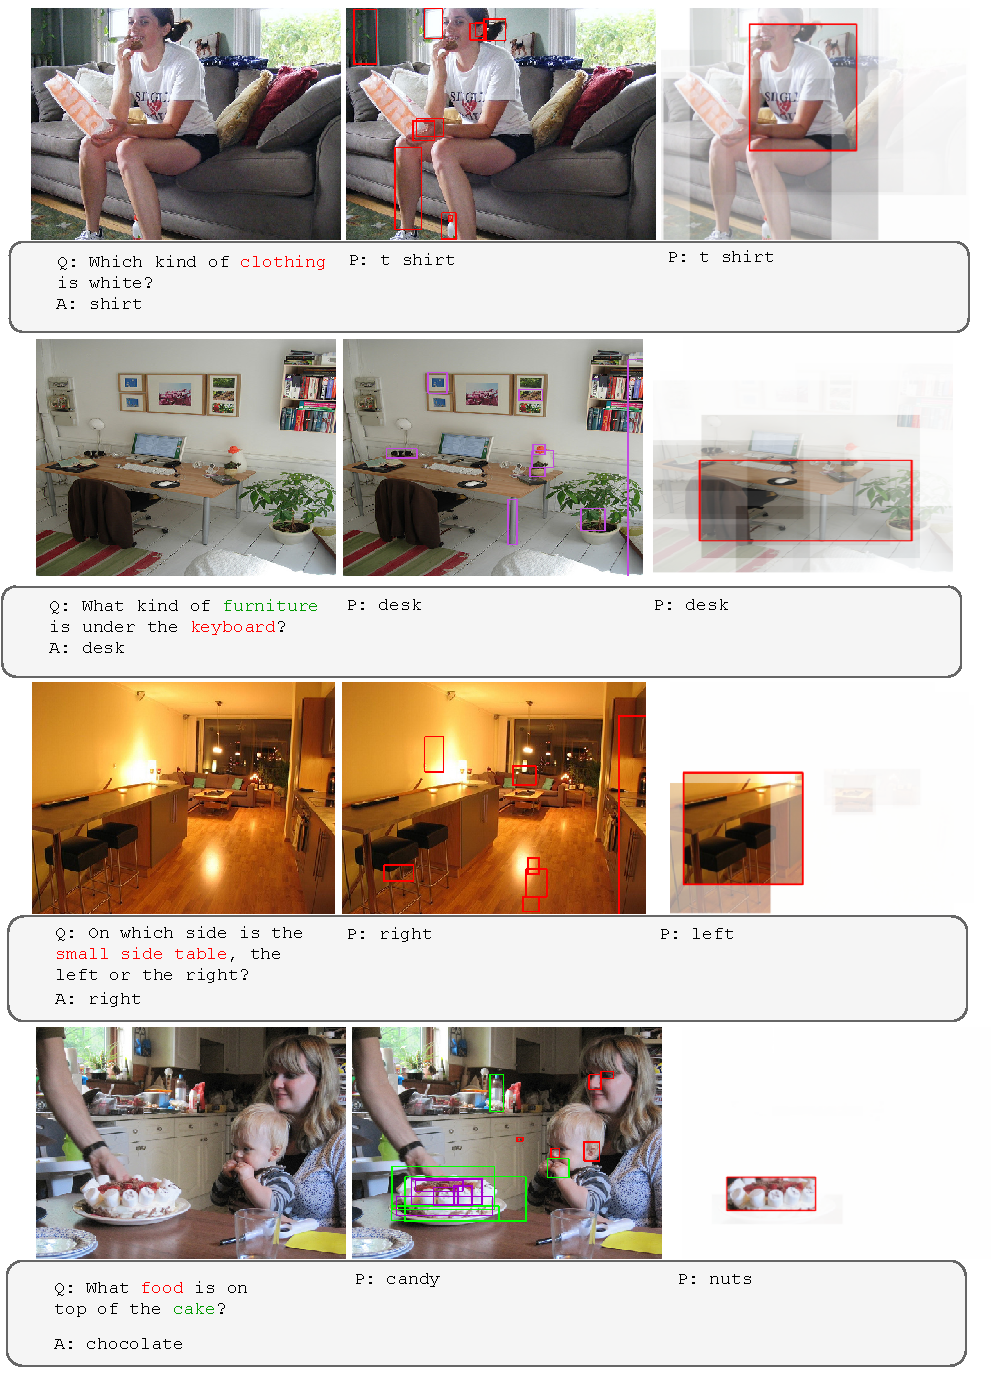
\includegraphics[scale=0.8]{att_visu}
	\caption{Examples of attention visualization for MCAN and ViLBERT on GQA \textit{testdev} set. From left to right are the original image-question pair, prediction and the learned image attention for multi-task ViLBERT, prediction and the learned image attention for MCAN. For ViLBERT, the bounding boxes correspond to the sentence to image attention of the highlighted words in the question. We use different bounding box color when the attention is shared between different words. As for MCAN, we visualize the attention learned by Eq. (\ref{eq_mcan_att}) and highlight the region with highest attention score.}
	\label{fig:att_visu}
\end{figure}

\section{Conclusion and Future Work}

\pagebreak
\bibliography{sempix}

\end{document}
